\section{Resultados} \label{resultados}

En esta sección se presentan los resultados obtenidos para cada una de las pruebas de verificación mencionadas en el apartado \ref{pruebas}. La elección de distintos parámetros de configuración que derivó de realizar pruebas preliminares no se discute aquí. Las decisiones tomadas son reportadas a lo largo de Materiales y Métodos, apartado \ref{materiales_metodos}.

\subsection{Desconexión y reconexión por USB del dispositivo}

Cuando el dispositivo se desconecta, un error de conexión es señalizado a la GUI desde el broker y fuerza a la terminación de este proceso. Si se está realizando una prueba, esta se detiene. Un recuadro que pide al usuario que reconecte el dispositivo aparece en pantalla, tal como se muestra en la Figura \ref{fig:UI-ESP-Disconected}. Si se conecta la ESP, el mensaje desaparece luego de presionar ``OK'' y se revierte el estado presentado en la Figura \ref{fig:UI-general-view}. Si se selecciona ``cancel'', la aplicación entra en modo de simulación.

\begin{figure}[H]
    \centering
    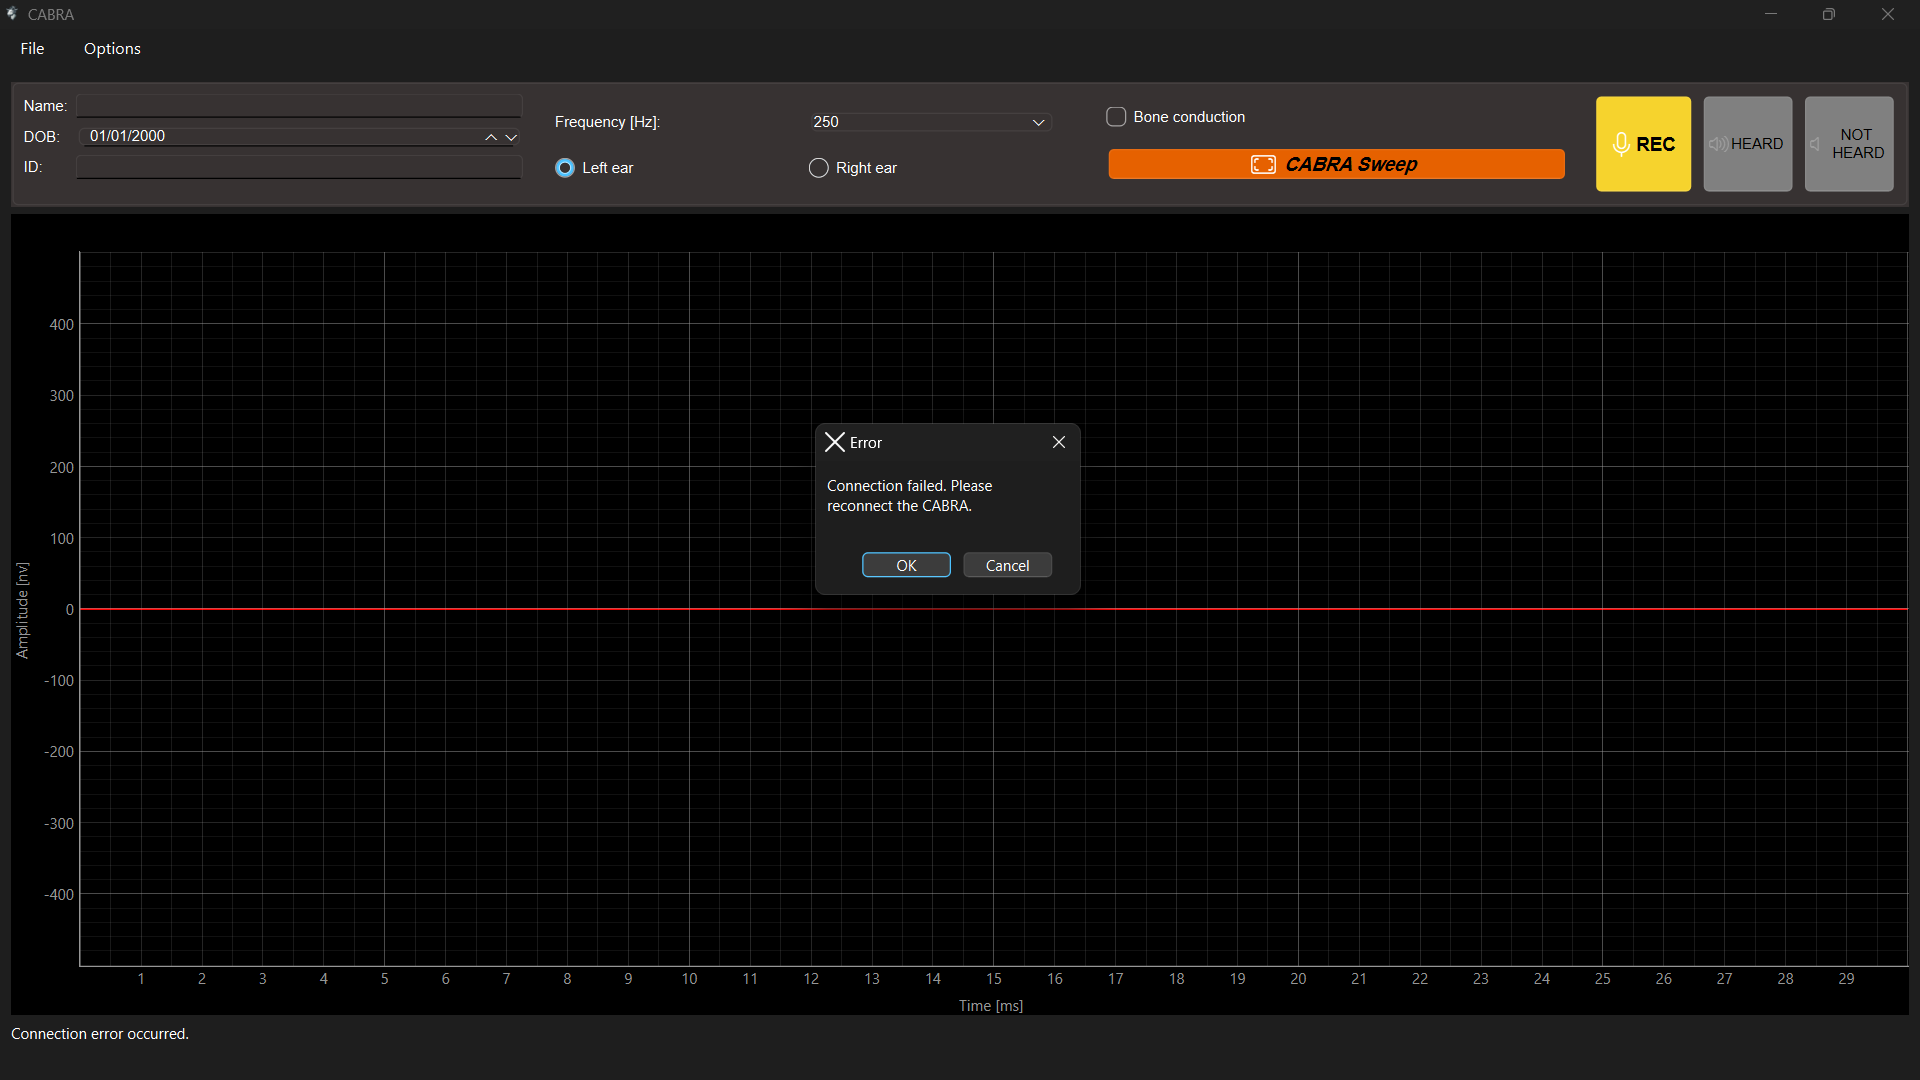
\includegraphics[width=1\linewidth]{figuras/UI-ESP-disconected.png}
    \caption{Cuadro de desconexión esperando acción del usuario. Notar el mensaje entregado en la barra de estado.}
    \label{fig:UI-ESP-Disconected}
\end{figure}

\subsection{Muestreo con el microcontrolador desconectado de la placa de preacondicionamiento}

Con el microcontrolador desconectado, podría esperarse visualizar una linea horizontal en torno a 0mV. No obstante, debido al ruido captado por el ADC, se observa una señal con una amplitud reducida, pero que está lejos de ser totalmente llana (ver Figura \ref{fig:UI-No-Board}). Tal como es de esperarse, el sistema experto sugiere que no hay presencia de percepción.

\begin{figure}[H]
    \centering
    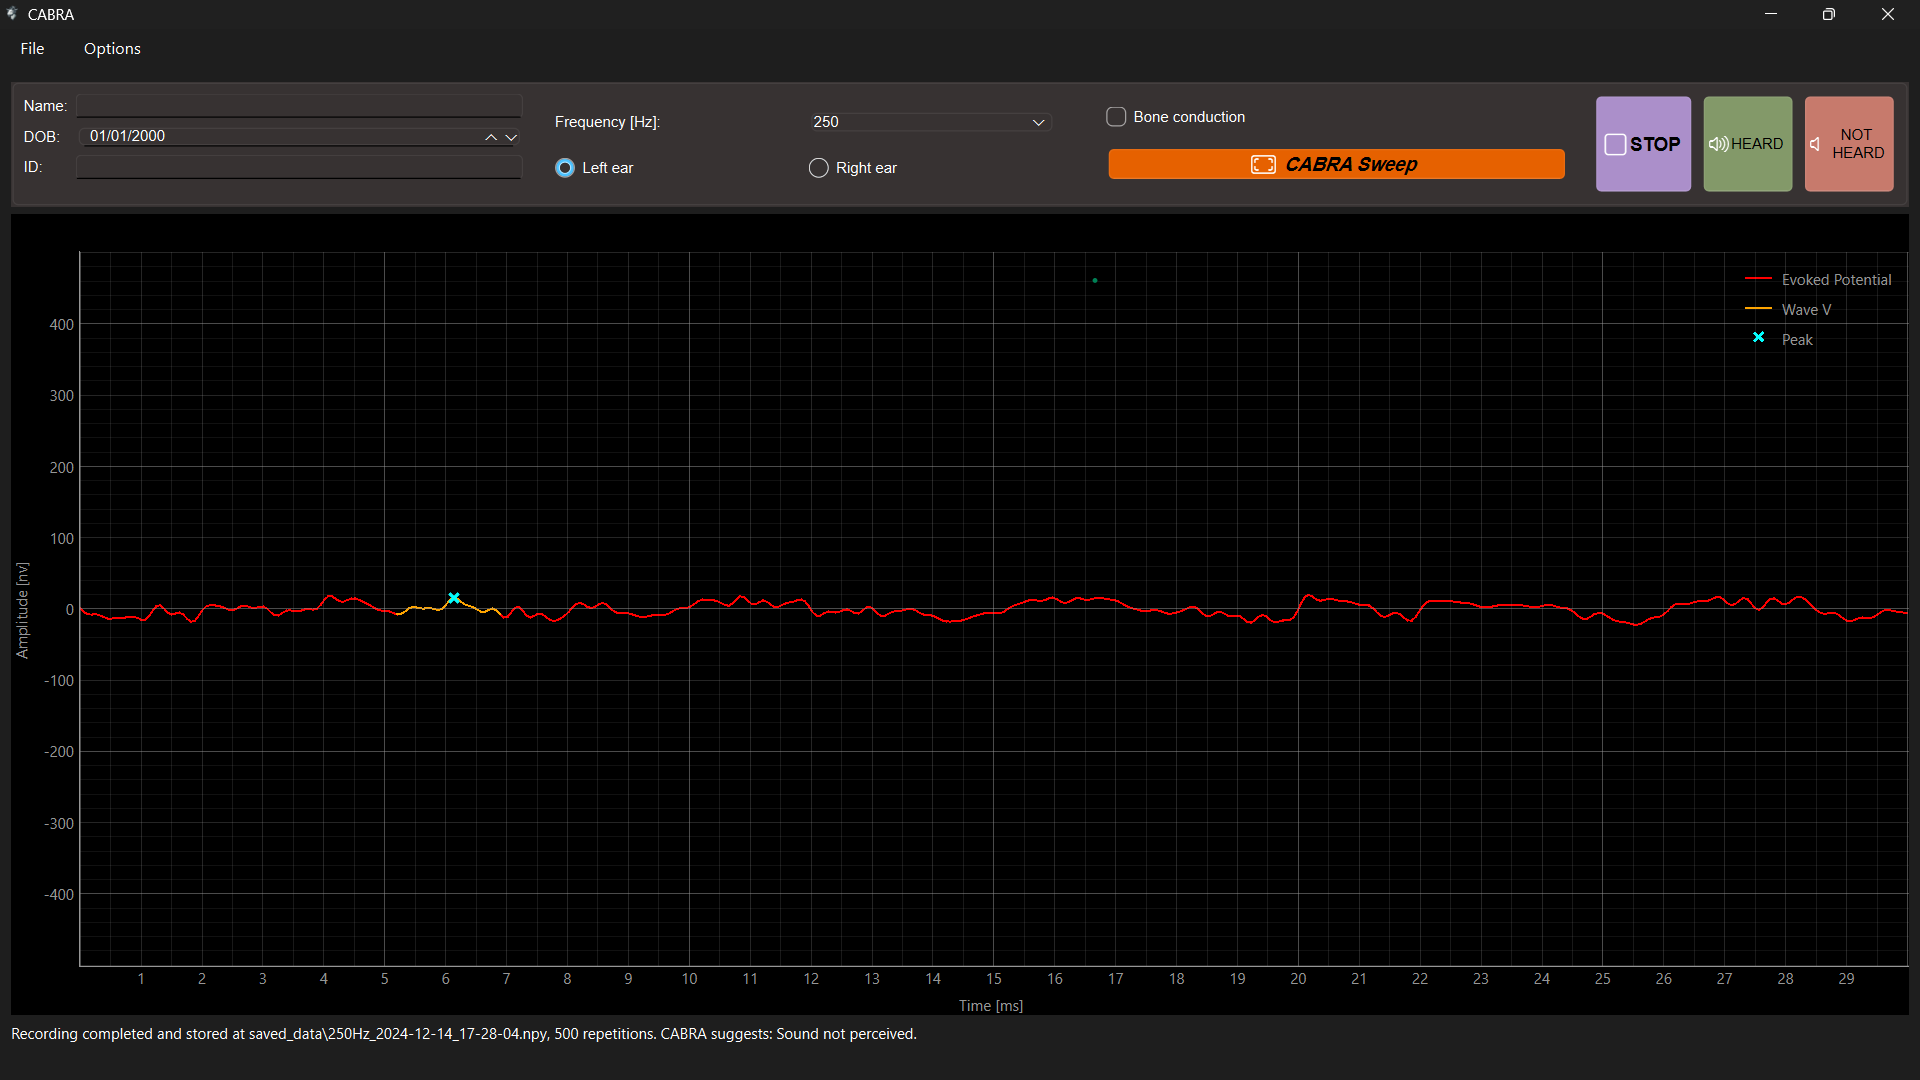
\includegraphics[width=1\linewidth]{figuras/UI-No-Board.png}
    \caption{Visualización de la señal obtenida por la ESP32 cuando no está conectada a la placa de adquisición.}
    \label{fig:UI-No-Board}
\end{figure}

Una prueba con mayor utilidad consiste en introducir una señal analógica con una frecuencia y amplitud conocidas, que permita testear el funcionamiento del protocolo de muestreo y el desempeño general del ADC. utilizando una senoidal a 100Hz, con 500mVpp y 1V de offset, logramos visualizar correctamente 3 ciclos cuando se pide un número de muestras equivalente a 30 ms.

\subsection{Muestreo con el paciente no conectado}

Cuando se conecta la ESP a la placa de adquisición y se realiza una prueba, lo más probable es que todas las repeticiones sean descartadas debido a que el sistema detecta que no se encuentran dentro del umbral de amplitud establecido, situación que puede ser visualizada en la Figura \ref{fig:UI-No-Patien}. Esto se debe a que los electrodos en este caso actúan como antenas y captan ruido electromagnético, que dada la gran ganancia del sistema se ve reflejado en una señal con una amplitud inusualmente grande. 

\begin{figure}[H]
    \centering
    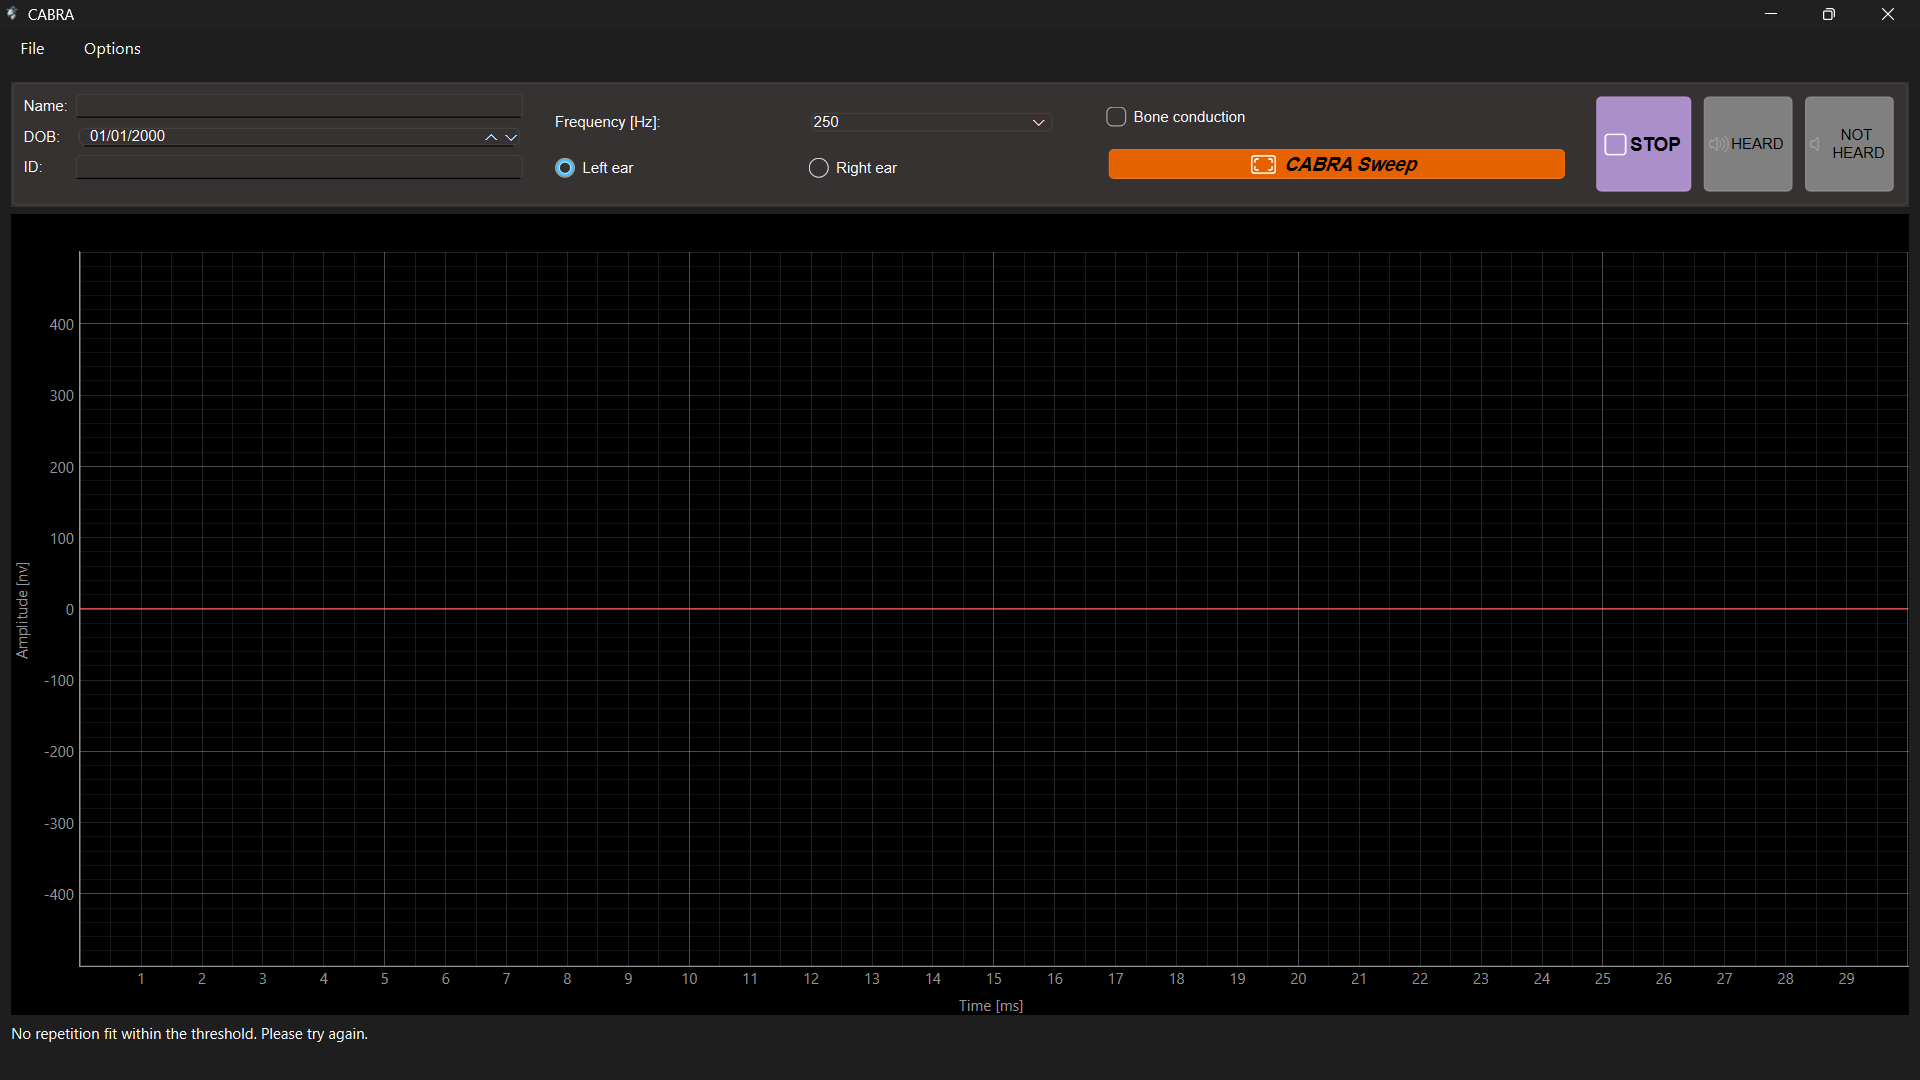
\includegraphics[width=1\linewidth]{figuras/UI-No-Patient.png}
    \caption{Mensaje de error indicado cuando no hay repeticiones que hayan entrado dentro del umbral correspondiente, situación común cuando el paciente no está conectado o está incorrectamente conectado.}
    \label{fig:UI-No-Patien}
\end{figure}

\subsection{Prueba con el paciente conectado, sin estímulo sonoro}

Cuando un paciente se conecta adecuadamente al dispositivo, pero no hay reacción neurofisiológica a los clicks, pero estos no están presentes, es posible observar una salida similar a lo observado en la Figura \ref{fig:UI-noise}. Notar que el sistema experto sugiere que no se percibió el estimulo, como era de esperarse.

\begin{figure}[H]
    \centering
    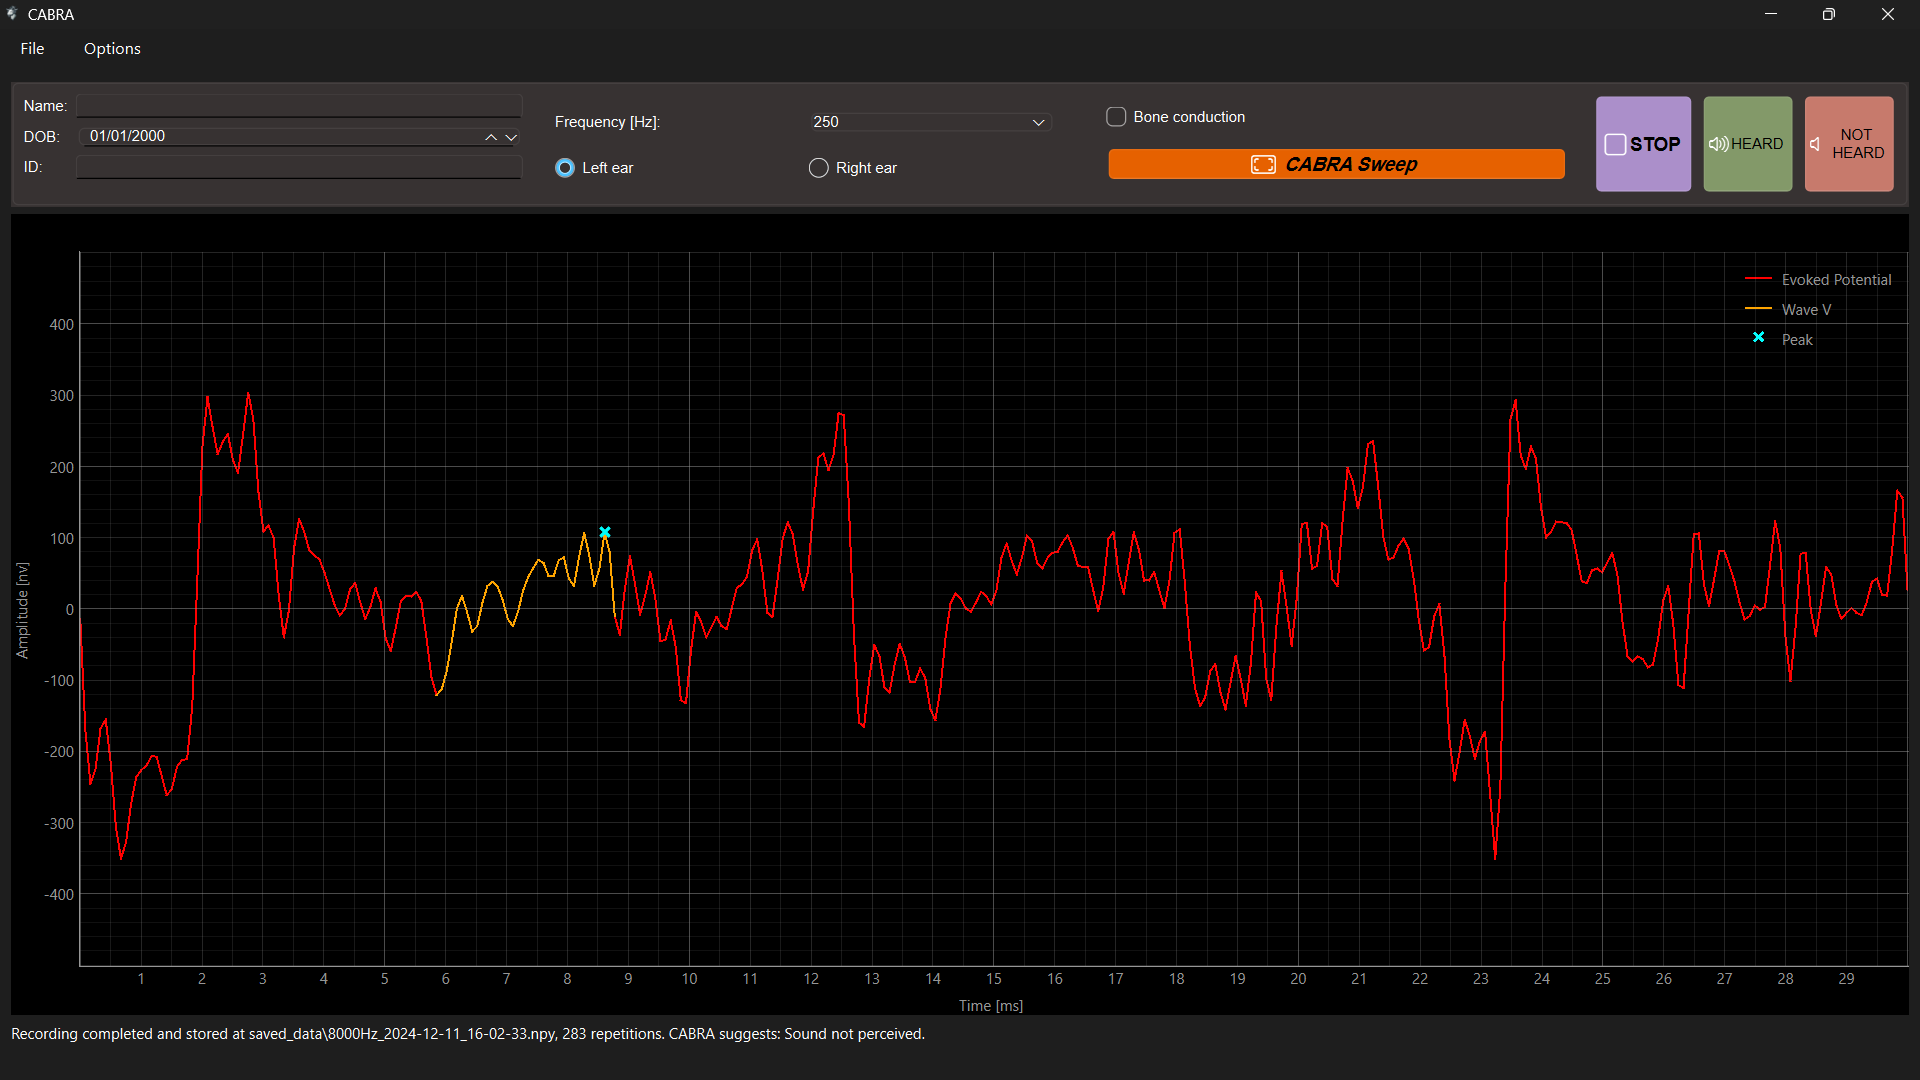
\includegraphics[width=1\linewidth]{figuras/UI-noise.png}
    \caption{Señal observada en una prueba en la que el sujeto de prueba no estaba escuchando clicks.}
    \label{fig:UI-noise}
\end{figure}

\subsection{Prueba con el paciente conectado, con estímulo sonoro reportado como perceptible}

El desenlace de una prueba en la que se reporta audición por parte del sujeto experimental se visualiza en la Figura \ref{fig:UI-EP}. Es importante mencionar que la calidad de la señal obtenida en este caso es fenomenal, con una morfología tipificada según literatura. No obstante, no logramos obtener en todas las pruebas los mismos resultados.

\begin{figure}[H]
    \centering
    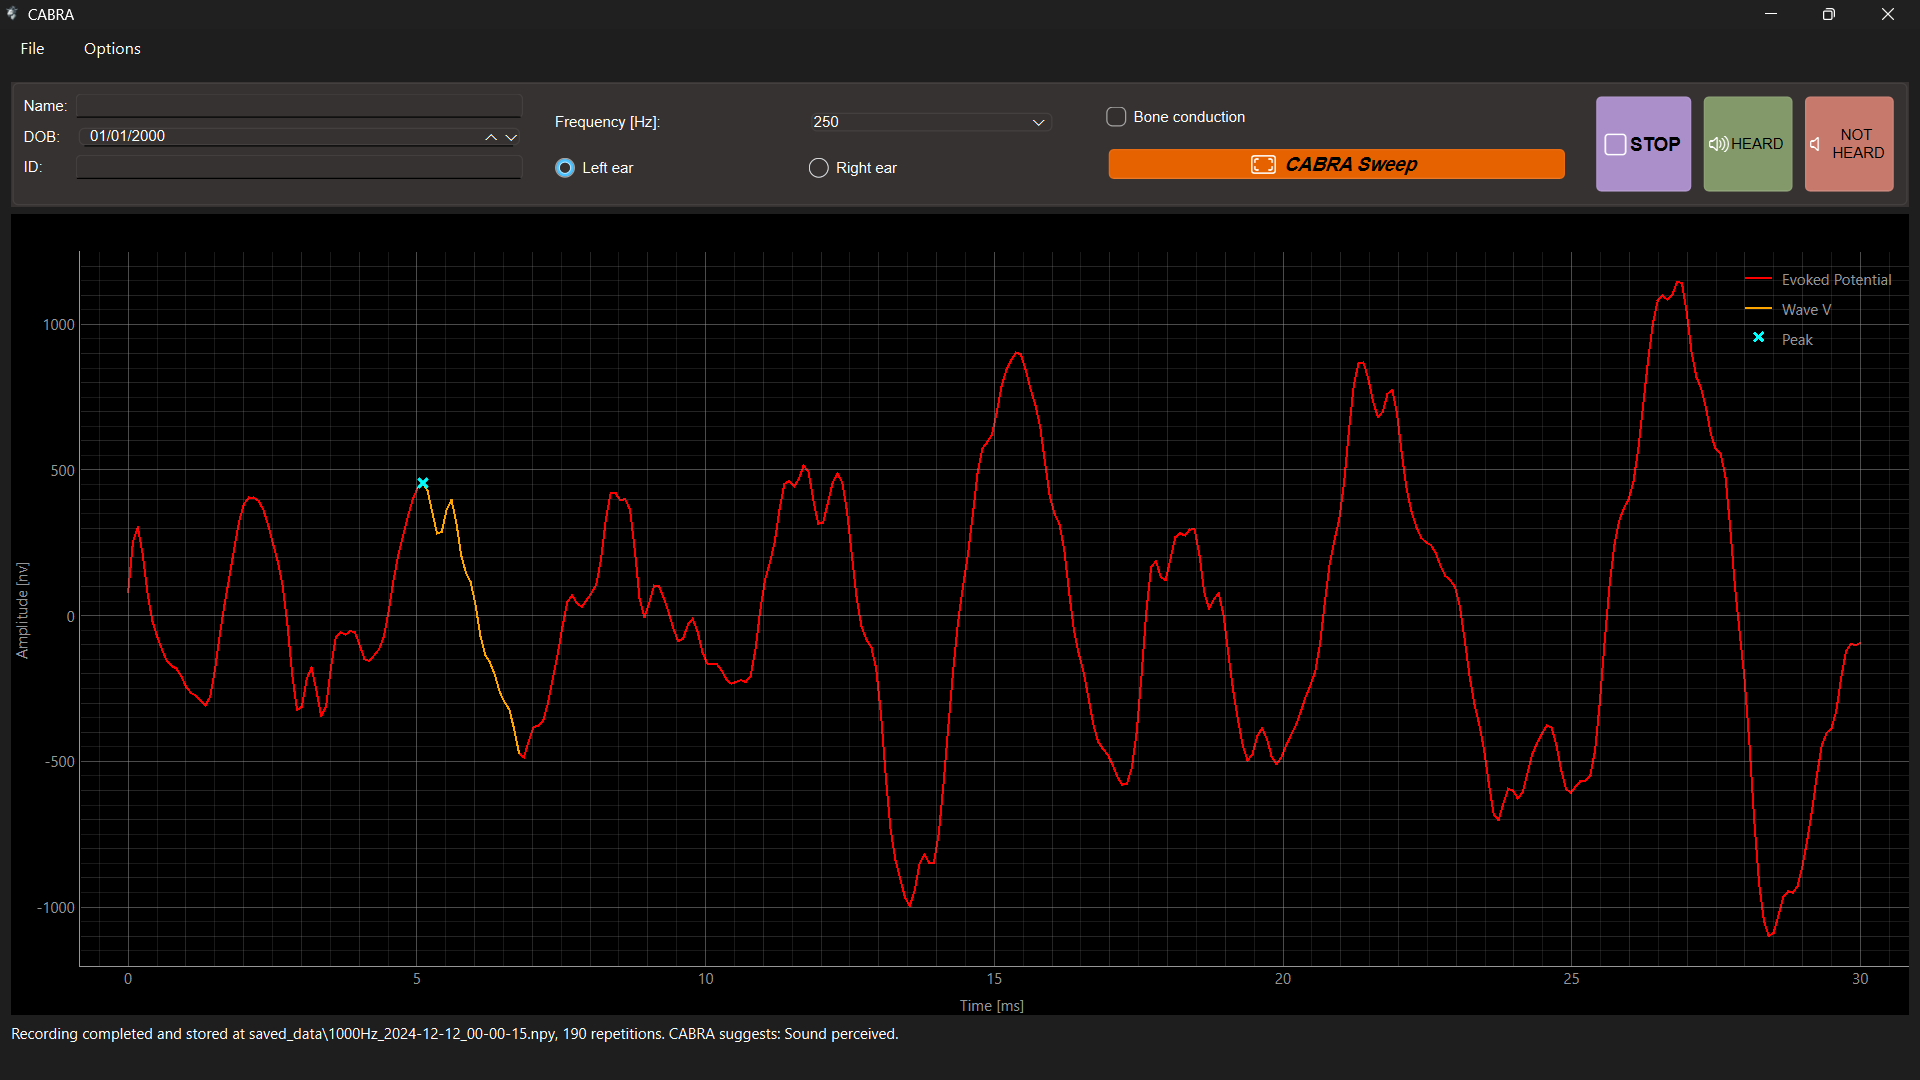
\includegraphics[width=1\linewidth]{figuras/UI-EP.png}
    \caption{Potencial evocado observado en una prueba en la que el sujeto de prueba reporta haber escuchado los clicks reproducidos. La descripción de la configuración utilizada se encuentra en la barra de estado.}
    \label{fig:UI-EP}
\end{figure}

\subsection{Simulación de una audiometría completa}

Tras ejecutar un test completo con un broker de datos que simula entregar potenciales evocados cuando la amplitud es mayor que el umbral dada una frecuencia y oído especificados, y ruido en caso contrario, se obtuvo la caracterización completa para un paciente ficticio cuyo perfil auditivo es relativamente usual (ver Figura \ref{fig:UI-complete-study}). Tanto los colores en la interfaz como los marcadores son los especificados por normativa internacional \cite{ISO389}.

\begin{figure}[H]
    \centering
    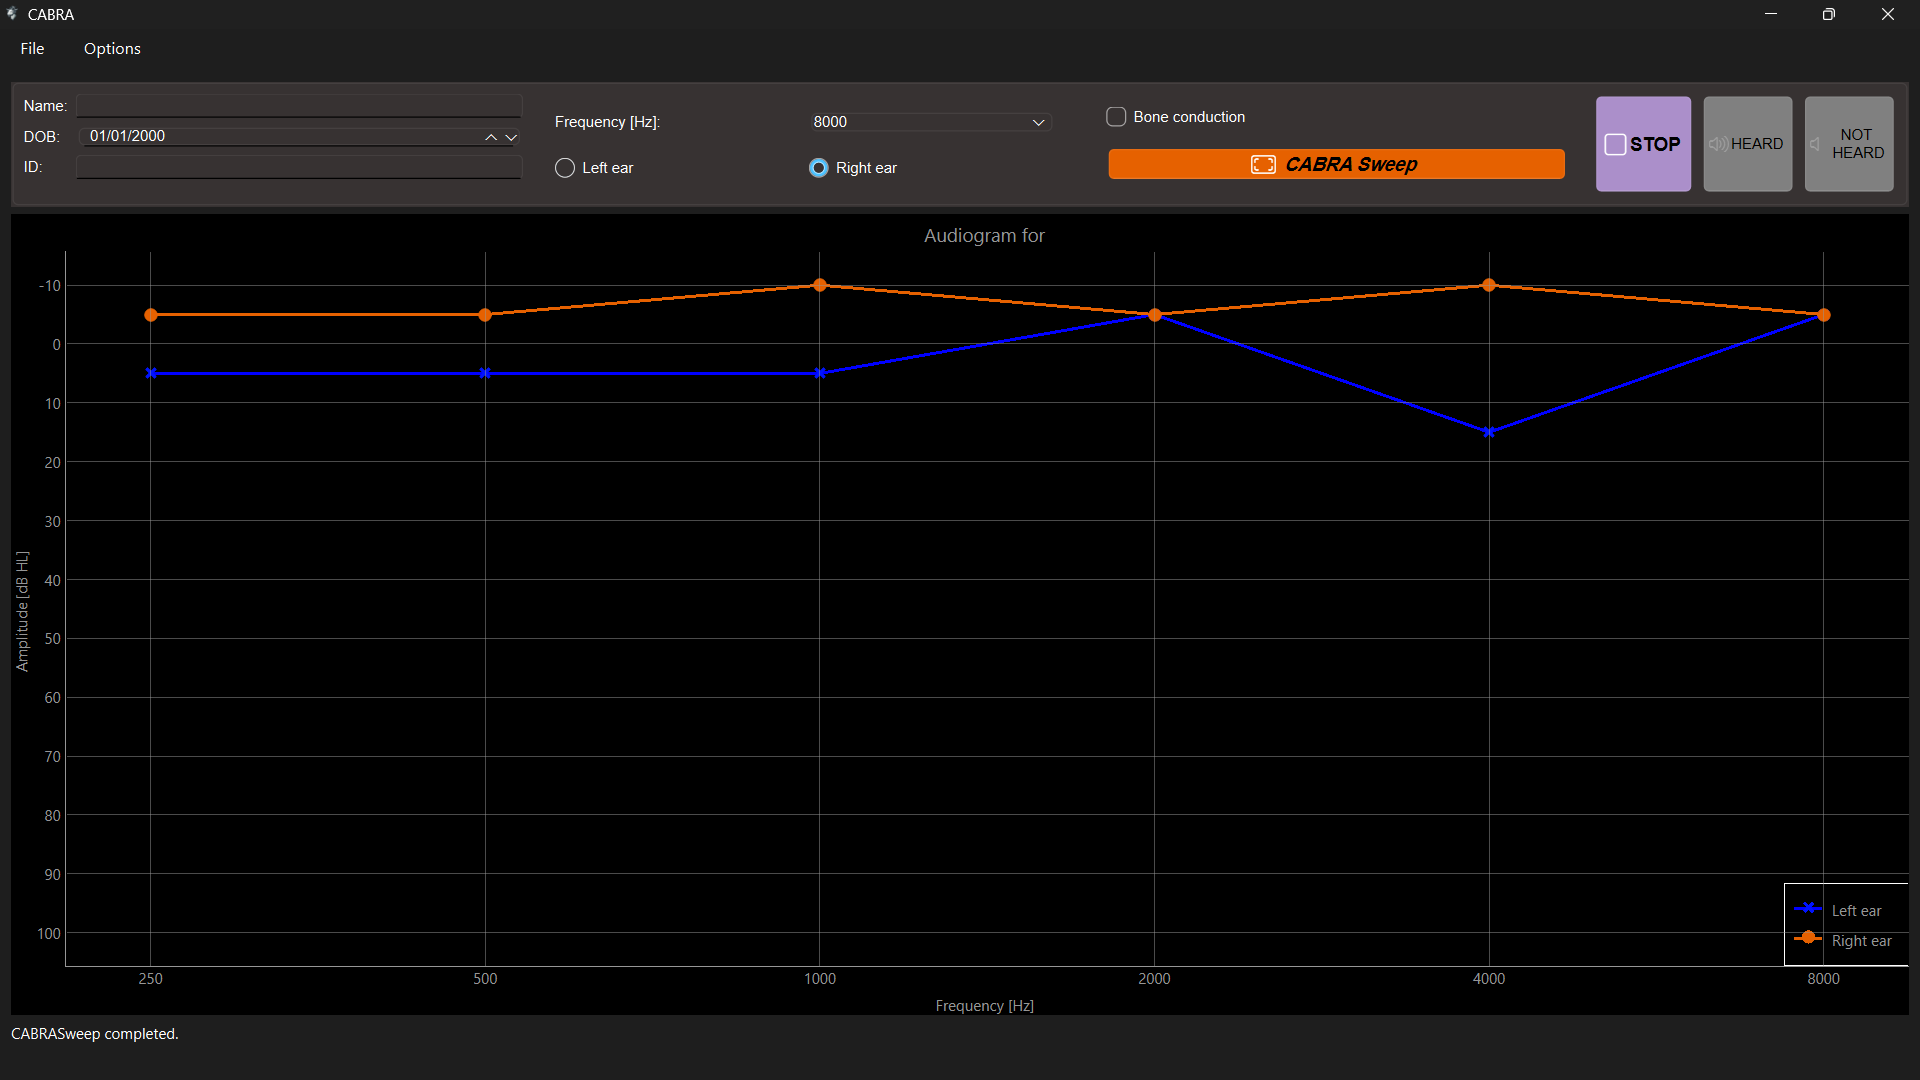
\includegraphics[width=1\linewidth]{figuras/UI-complete-study.png}
    \caption{Visualización de audiometría completa simulada, realizada con el algoritmo de búsqueda de la aplicación y CABRA \textit{Sweep}.}
    \label{fig:UI-complete-study}
\end{figure}